
\chapter{MỞ ĐẦU}
\label{Introduction}

\section{Bối cảnh chung}

\begin{figure}[h!]
  \centering
  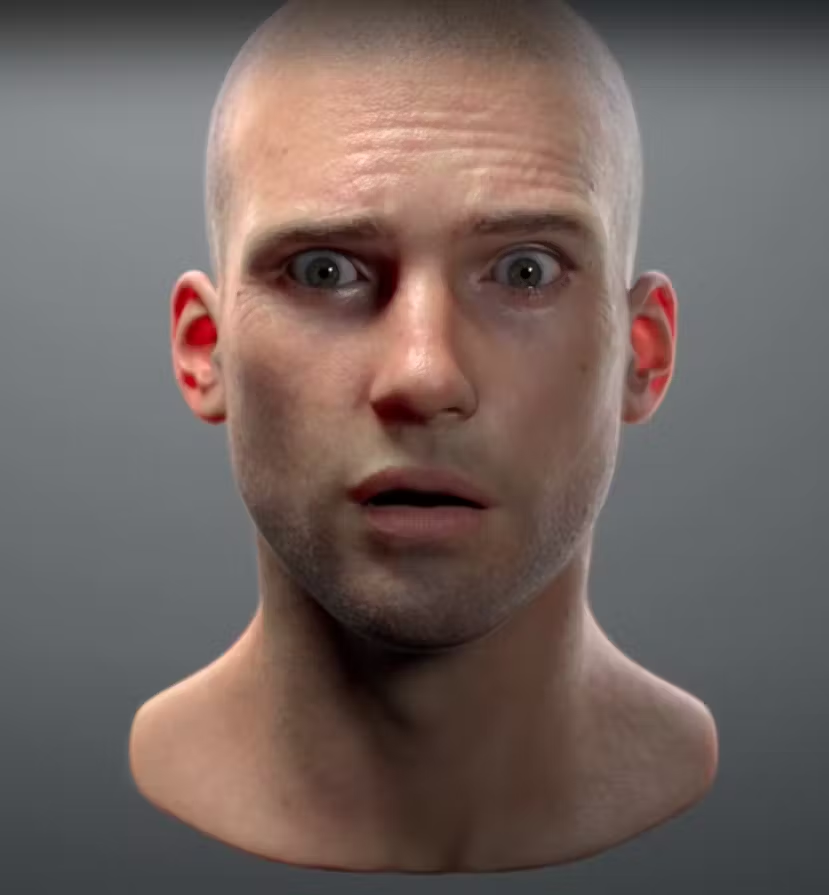
\includegraphics[width=0.5\linewidth]{cgi.png}
  \caption{Công nghệ CGI với người kỹ thuật số siêu thật \cite{edchrisjones}}
  \label{fig:cgi}
\end{figure}

Mỗi ngày, trên thế giới có hàng tỷ người nhìn vào màn hình RGB, kết quả hiển thị trên màn hình là đầu ra của mọi hệ thống phần mềm, nên việc hiển thị từng pixel trên màn hình và cách để mô phỏng lại hình ảnh trên một cách chân thực nhất được các nhà khoa học về đồ họa máy tính (Computer Graphic) nghiên cứu từ những năm 1960s và đặc biệt là việc mô hình phỏng lại con người. Từ 2014, các hoạ sĩ 3d đã có thể tạo nên một nhân vật người siêu thật như \autoref{fig:cgi} trong khi các phần cứng máy tính còn chưa phát triển như hiện nay. 

Ngày nay, công nghệ đồ họa máy tính đã hoàn toàn có thể mô phỏng nhiều vật giống đến mức siêu thực (realistic) các vật phức tạp như nước, đường xá, bánh mỳ,...  và thậm chí là cả cơ thể và khuôn mặt con người với độ chi tiết đến từng lông tơ, nốt mụn và vân mắt. 
Vào năm 2015, bằng kỹ thuật quyét 3 chiều ghi lại toàn bộ các góc của khuôn mặt, sự phản chiếu ánh sáng, trong công trình \cite{metallo2015scanning}
nhà khoa học đồ họa máy tính đã có thể tái tạo toàn bộ khuôn mặt của tổng thống Obama trên máy tính với độ chính xác cao và gần như không thể phân biệt \autoref{fig:obamascan}.

\begin{figure}[H]
    \centering
    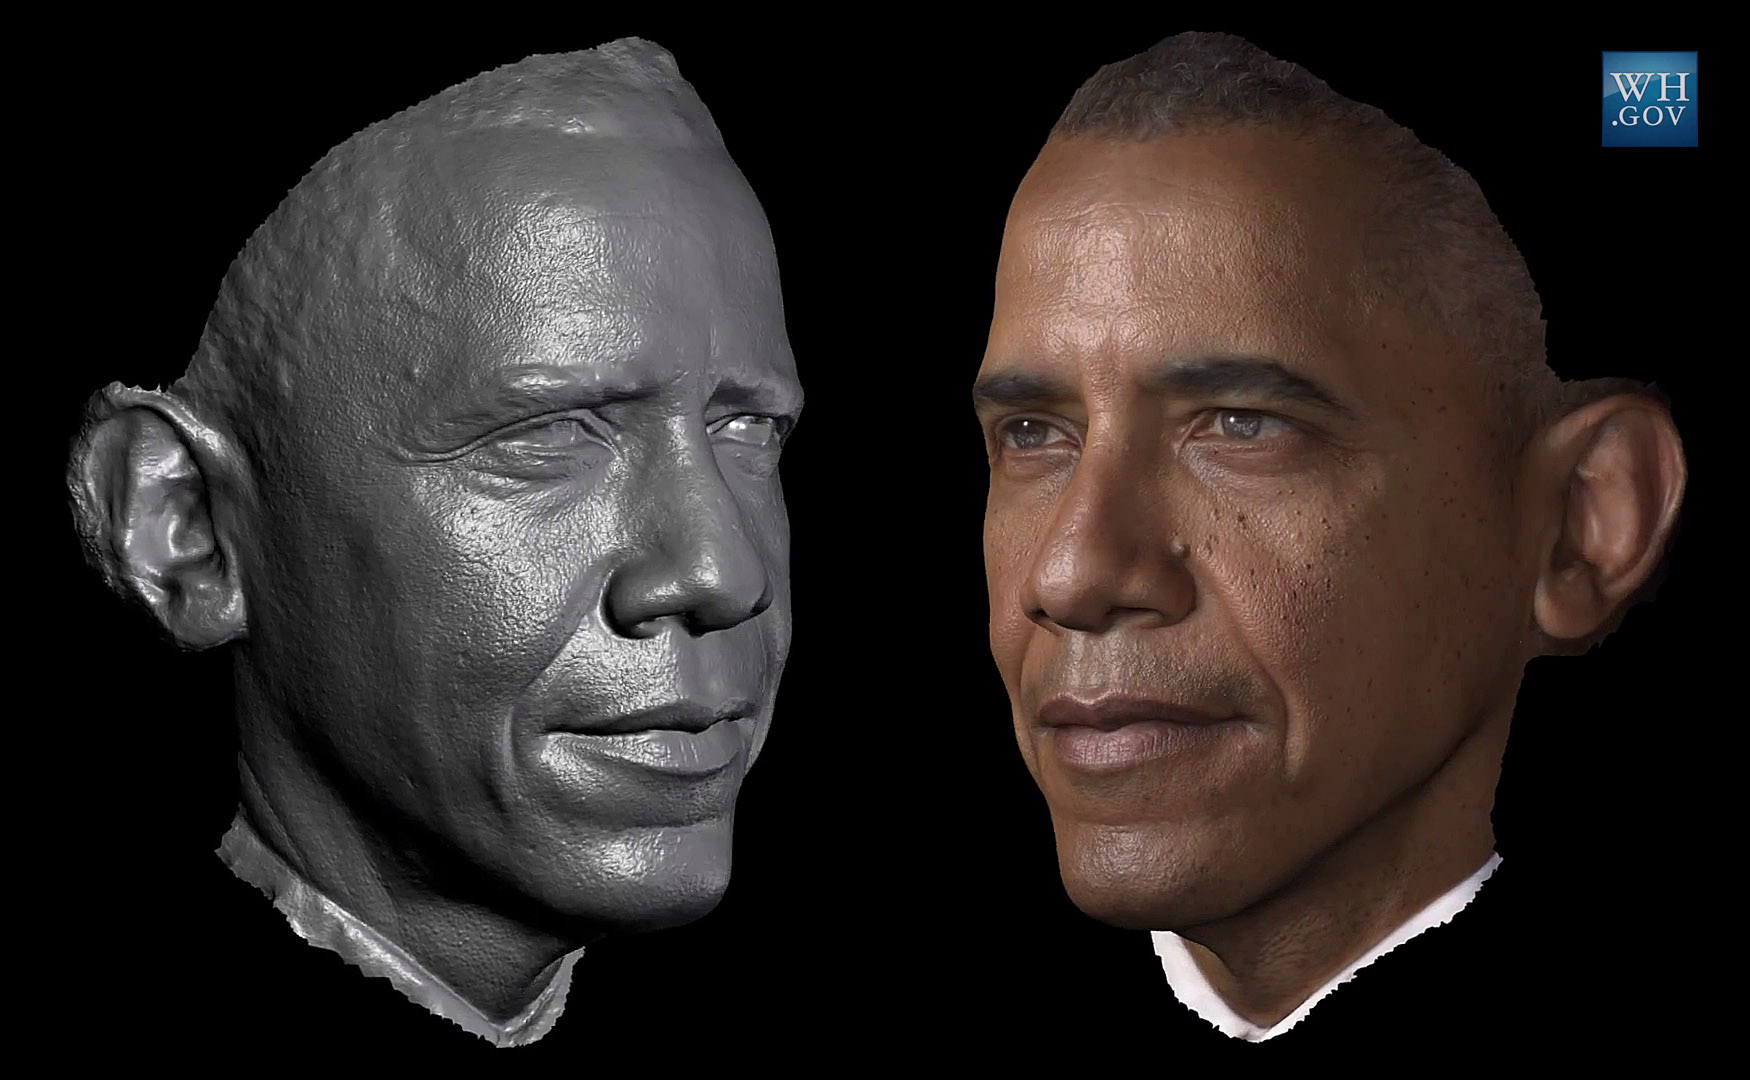
\includegraphics[width=\linewidth]{obama_scan.jpg}
    \caption{Minh họa công trình tái tạo khuôn mặt tổng thống Obama \cite{metallo2015scanning} }
    \label{fig:obamascan}
\end{figure}

Trí tuệ nhân tạo thể hiện kết quả vượt bậc những năm gần đây không chỉ trong nghiên cứu mà con trong ứng dụng thực tế, tiêu biểu như ứng dụng ChatGPT, Midjouney và sự phát triển cả theo chiều dọc và chiều ngang trong việc ứng dụng trí tuệ nhân tạo với nhiều lĩnh vực khác nhau. Mặc dù đồ họa máy tính đã có thể xây dựng khuôn mặt người siêu thật, việc sinh cử chỉ lại phụ thuộc vào việc Chụp chuyển động (Motion Capture) từ các cảm biến và gặp rất nhiều khó khăn khi xây dựng một hệ thống trí tuệ nhân tạo để học từ dữ liệu.

Các hệ thống trí tuệ nhân tạo hiện nay đã có thể tạo văn bản và âm thanh tiệm cận như con người, nhưng một trong những trở ngại lớn nhất để xây dựng con người kỹ thuật số hiện nay chính là việc sinh cử chỉ. Chính vì vậy mà mục tiêu của luận văn là xây dựng một hệ thống sinh cử chỉ hội thoại dựa trên cảm xúc và ngữ nghĩa với dữ liệu đầu vào gồm cả văn bản và giọng nói.

\section{Động lực nghiên cứu}

% Ý nghĩa khoa học và ứng dụng của đề tài
% Vai trò của việc sinh cử chỉ
Tổng hợp cử chỉ hội thoại giúp ích cho rất nhiều lĩnh vực như hoạt ảnh, dựng phim, trò chơi điện tử, giáo dục và những ứng dụng thực tại ảo. Việc tổng hợp cử chỉ chuyển động được thực hiện theo cách truyền thống là thuê các diễn viên sử dụng các tracker và bố trí các hệ thống cảm biến xung quanh thu nhận chuyển động để đạt được độ chính xác nhân thực nhất. Tuy nhiên, các chuyển động thu được sau đó chỉ được phát lại và không có sự biến chuyển giữa các hành động hay chuyển động, chính vì vậy, việc áp dụng trí tuệ nhân tạo để có thể học các chuyển động từ dữ liệu thu nhận và sau đó có thể sinh ra dữ liệu mới sẽ là một cuộc cách mạng trong ngành công nghiệp Motion Capture.

Vào năm 2011, một nhóm tác giả \cite{bergmann2011relation} đã chứng minh rằng có sự liên hệ giữa giọng nói và cử chỉ con người, đây chính là tiền đề để cho thấy chúng ta có thể dùng dữ liệu âm thanh để có thể dùng để học và biểu diễn được cử chỉ con người.
Với sự thành công của các mô hình ngôn ngữ tự nhiên trong việc xử lý ngôn ngữ văn bản, với sự chính xác siêu thật trong việc mô phỏng gương mặt con người trong lĩnh vực Đồ họa máy tính và với sự chính xác và dễ dàng từ việc tổng hợp giọng nói con người hiện nay. Thì việc ứng dụng trí tuệ nhân tạo để sinh cử chỉ con người là một trong những điểm nghẽn cổ chai duy nhất trong việc phát triển một trợ lý ảo để trao đổi và tương tác với con người.

\section{Phát biểu bài toán}

Mục tiêu của việc sinh cử chỉ (gesture generation) bằng phương pháp học máy là tạo ra các cử chỉ tự nhiên, chân thật như con người (human-likeness) và đồng thời phù hợp với ngữ cảnh.
%Sinh cử chỉ (gesture generation) là bài toán dựa vào những dữ liệu trước đó bao gồm văn bản và âm thanh, cử chỉ khởi tạo để nội suy ra chuỗi cử chỉ tiếp theo.
Sinh cử chỉ là bài toán hồi quy (regression), với đầu vào là một chuỗi cử chỉ cho trước và kết quả đầu ra là chuỗi cử chỉ tiếp tục với cử chỉ trước đó.


\begin{figure}[htbp]
	\centering
	\begin{subfigure}{0.49\textwidth}
		\centering
		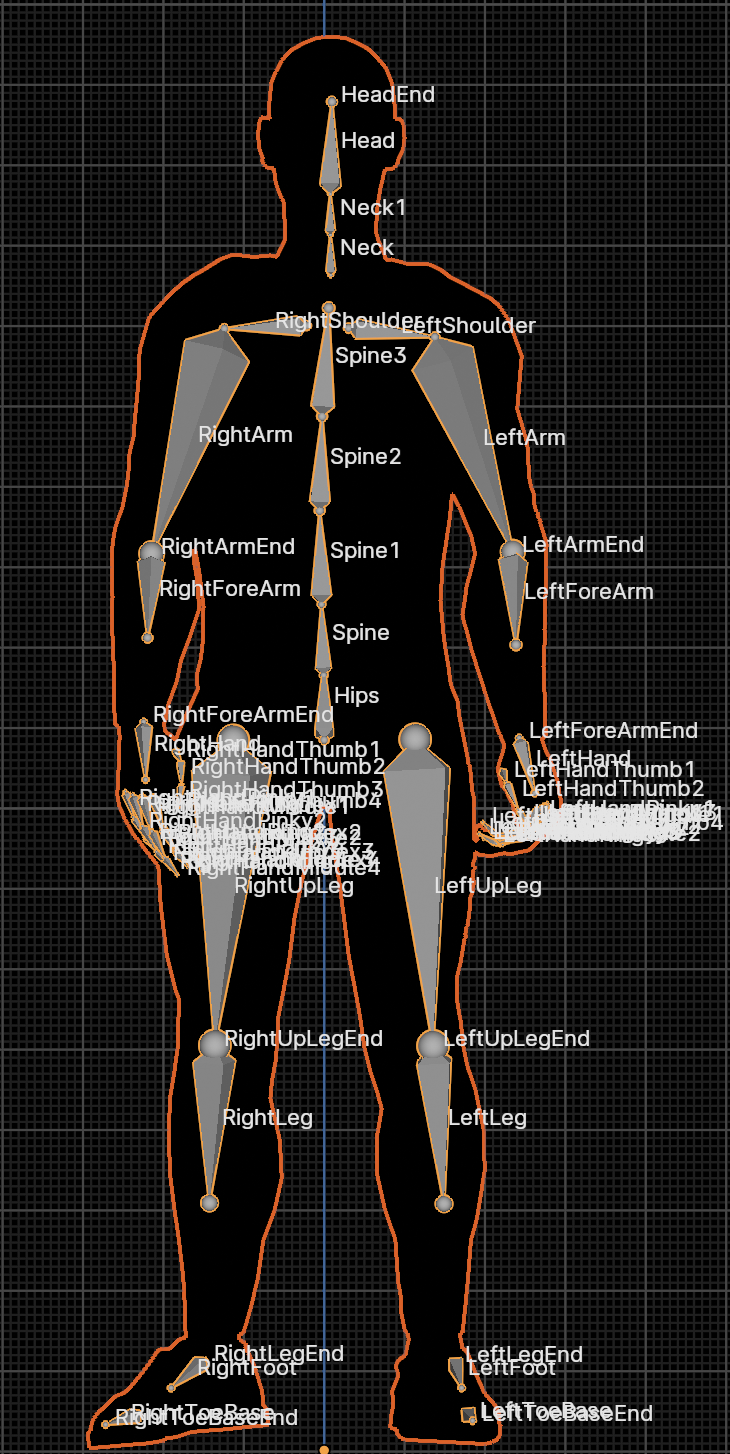
\includegraphics[height=10cm]{images/Skeleton.png}
		\caption{\small Khung xương và tên của các khớp của một khung xương trong mỗi khung hình.}
		\label{fig:Skeleton}
	\end{subfigure}
	\hfill
	\begin{subfigure}{0.49\textwidth}
		\centering
		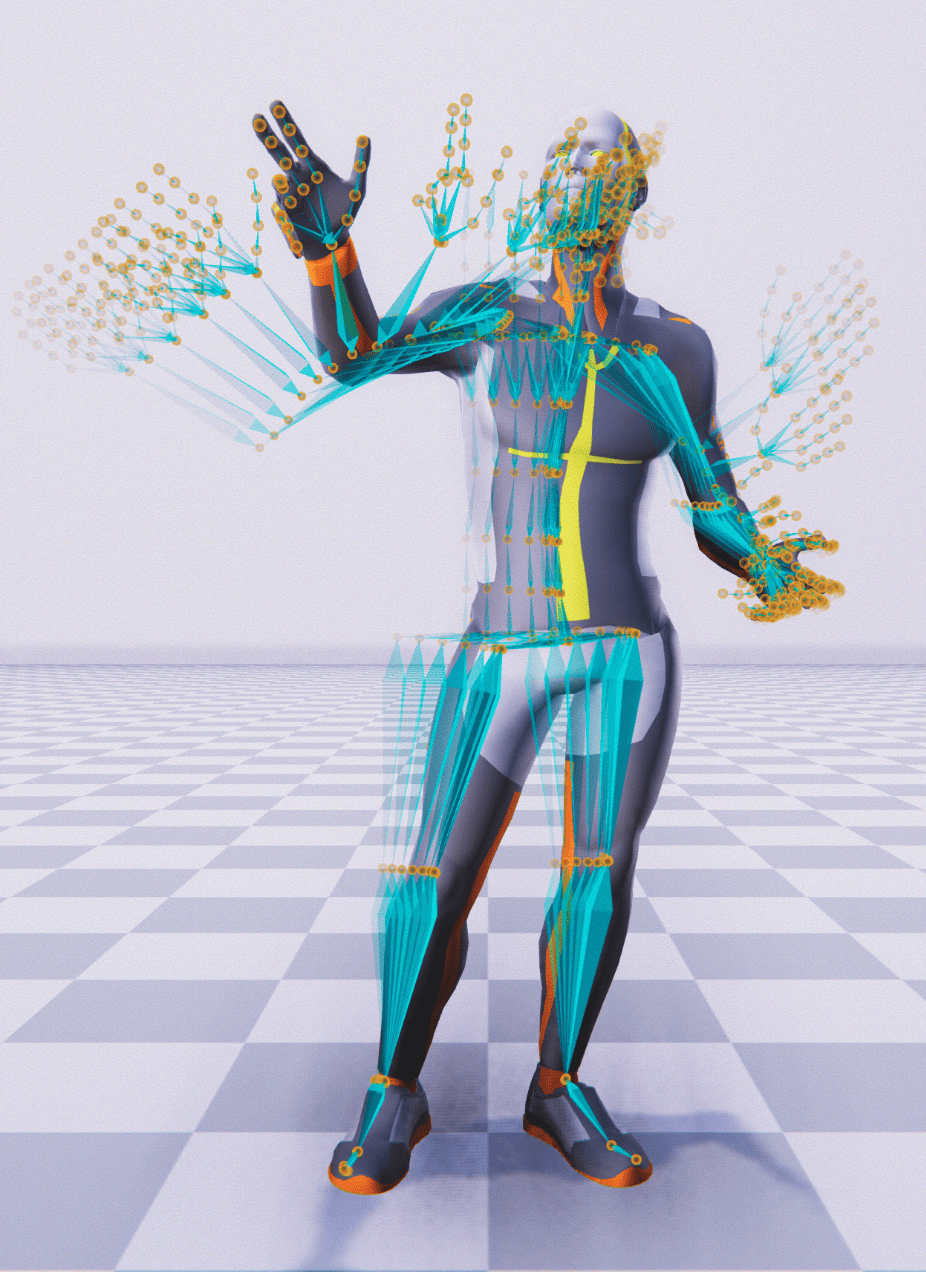
\includegraphics[height=10cm]{images/MotionPastAndFuture.png}
		\caption{\small Chuỗi chuyển động của cử chỉ bao gồm 6 cử chỉ quá khứ và 6 cử chỉ tương lai.}
		\label{fig:MotionPastAndFuture}
	\end{subfigure}
\end{figure}

Mỗi khung hình chuyển động của một nhân vật hay khung xương (skeleton) bao gồm dữ liệu về toạ độ vị trí và vận tốc theo thời gian.
Ở đây dữ liệu của chúng tôi của một khung xương với mỗi khung hình (frame) bao gồm:

\begin{equation} \label{eq:gesturevector}
\mathbf{g} = \Big[ \mathbf{p}_{\text{root}},  \mathbf{r}_{\text{root}},
\mathbf{ p }'_{\text{root}},  \mathbf{r}'_{\text{root}},
\mathbf{p}_{\text{joins}},  \mathbf{r}_{\text{joins}},
\mathbf{p}'_{\text{joins}},  \mathbf{r}'_{\text{joins}},
\mathbf{d}_{\text{gaze}}
\Big]
\end{equation}



Trong  đó với mỗi $\mathbf{g} \in \mathbb{R}^{1141}$ bao gồm:
{
\begin{itemize}
	\item $\mathbf{p}_{\text{root}} \in \mathbb{R}^3$: Toạ độ của điểm gốc
	\item $\mathbf{r}_{\text{root}} \in \mathbb{R}^4$: Góc quay của điểm gốc
	\item $\mathbf{p}'_{\text{root}} \in \mathbb{R}^3$: Vận tốc thay đổi của toạ độ gốc
	\item $\mathbf{r}'_{\text{root}} \in \mathbb{R}^3$: Vận tốc thay đổi của góc quay gốc
	
	\item $\mathbf{p}_{\text{joins}} \in \mathbb{R}^{3 n_{\text{join} }}$: Toạ độ của các khung xương
	\item $\mathbf{r}_{\text{joins}} \in \mathbb{R}^{6 n_{\text{join} }}$: Góc quay của các khung xương theo mặc phẳng X và Y
	\item $\mathbf{p}'_{\text{joins}} \in \mathbb{R}^{3n_{\text{join} }}$: Vận tốc thay đổi của toạ độ các khung xương
	\item $\mathbf{r}'_{\text{joins}} \in \mathbb{R}^{3n_{\text{join} }}$: Vận tốc thay đổi của góc quay các khung xương
	\item $\mathbf{d}_{\text{gaze}} \in \mathbb{R}^3$: Là hướng nhìn
\end{itemize}}


%\begin{figure}
%	\centering
%	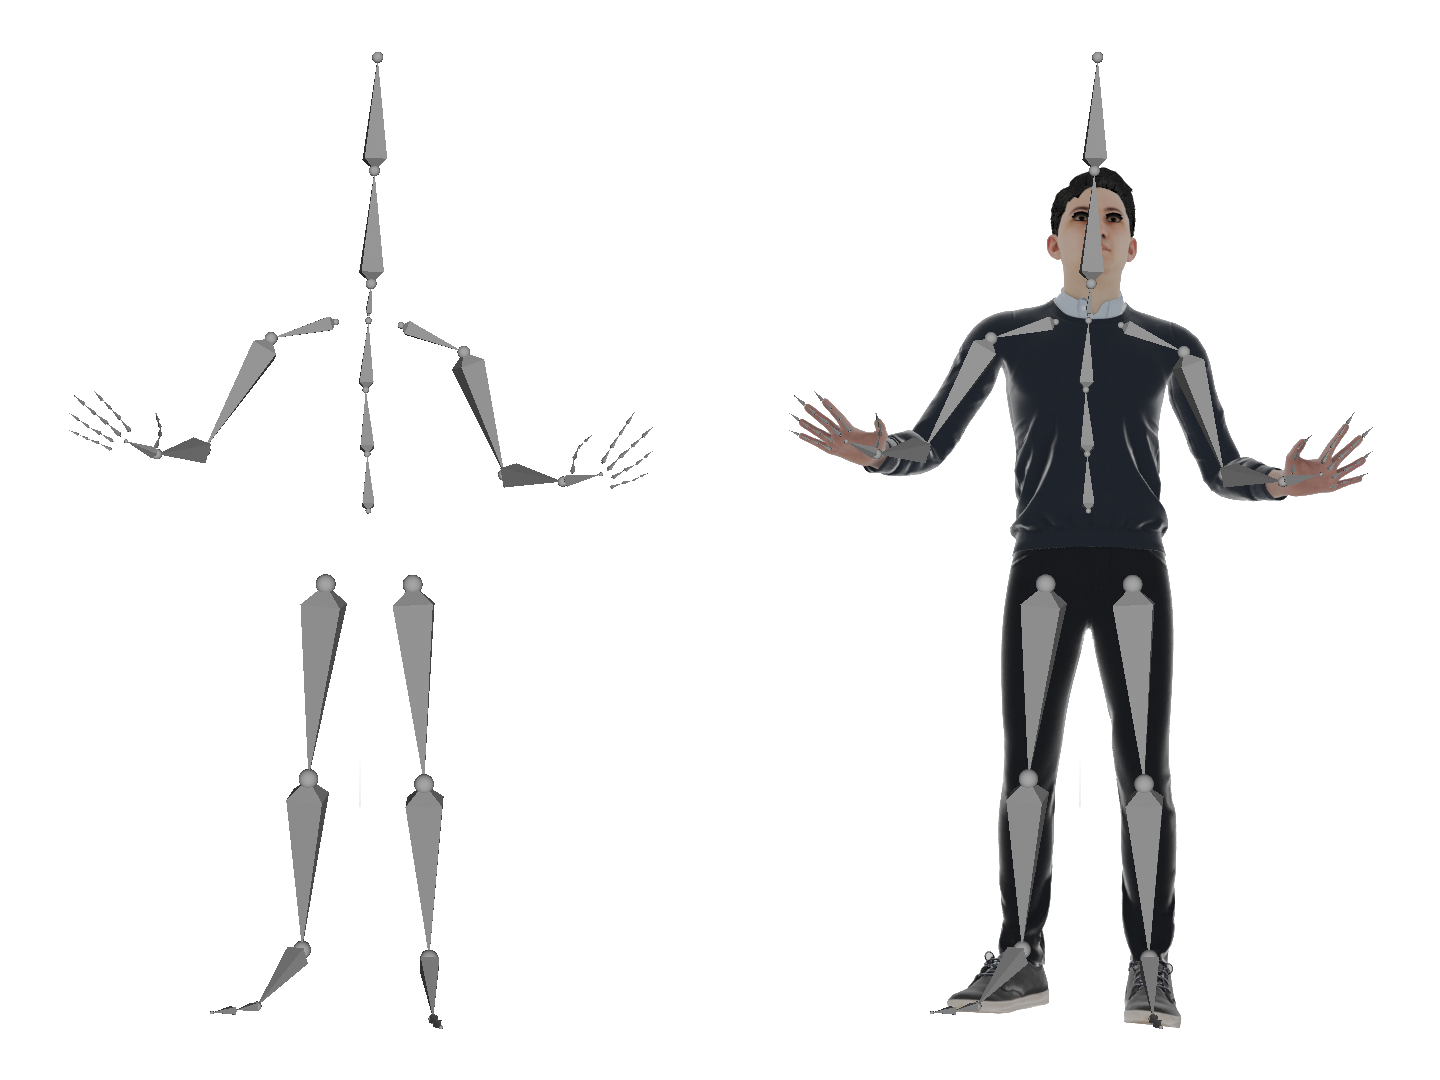
\includegraphics[width=0.8\linewidth]{images/skeleton_sample.png}
%	\caption{Minh họa một cử chỉ và mô hình nhân vật}
%	\label{fig:software}
%\end{figure}


Tổng cộng có $75$ khớp (joins) hay $n_{\text{join}} = 75$, với mỗi khung hình (frame) ta sẽ có một vector gồm 1141 chiều.
Tập dữ liệu là tập nhiều chuỗi cử chỉ với độ dài tuỳ ý, từ mỗi cử chỉ độ dài tuỳ tý ta sẽ cắt thành các đoạn $N + M$ khung hình, $g \in \mathbb{R}^{(N + M) \times 1141}$ , trong đó cử chỉ $\mathbf{s} \in \mathbb{R}^{N \times 1141}$ đầu tiên là cử chỉ khởi tạo (seed gesture), $\bx \in \mathbb{R}^{M \times 1141}$ cử chỉ tiếp theo cho việc dự đoán.


Dữ liệu âm thanh $\mathbf{a}_{\text{raw}} \in \mathbb{R}^{ \text{length } }$ là chuỗi âm thanh thô được đọc ở sample rate 16000, sau đó được cắt thành $\mathbf{a} \in \mathbb{R}^{64000}$ tương ứng với 4 giây.
% để  là một chuỗi waveform có độ dài tương ứng với cử chỉ được đọc với sample rate là 16000. 
\setcounter{figure}{2}
\begin{figure}[H]
	\centering
	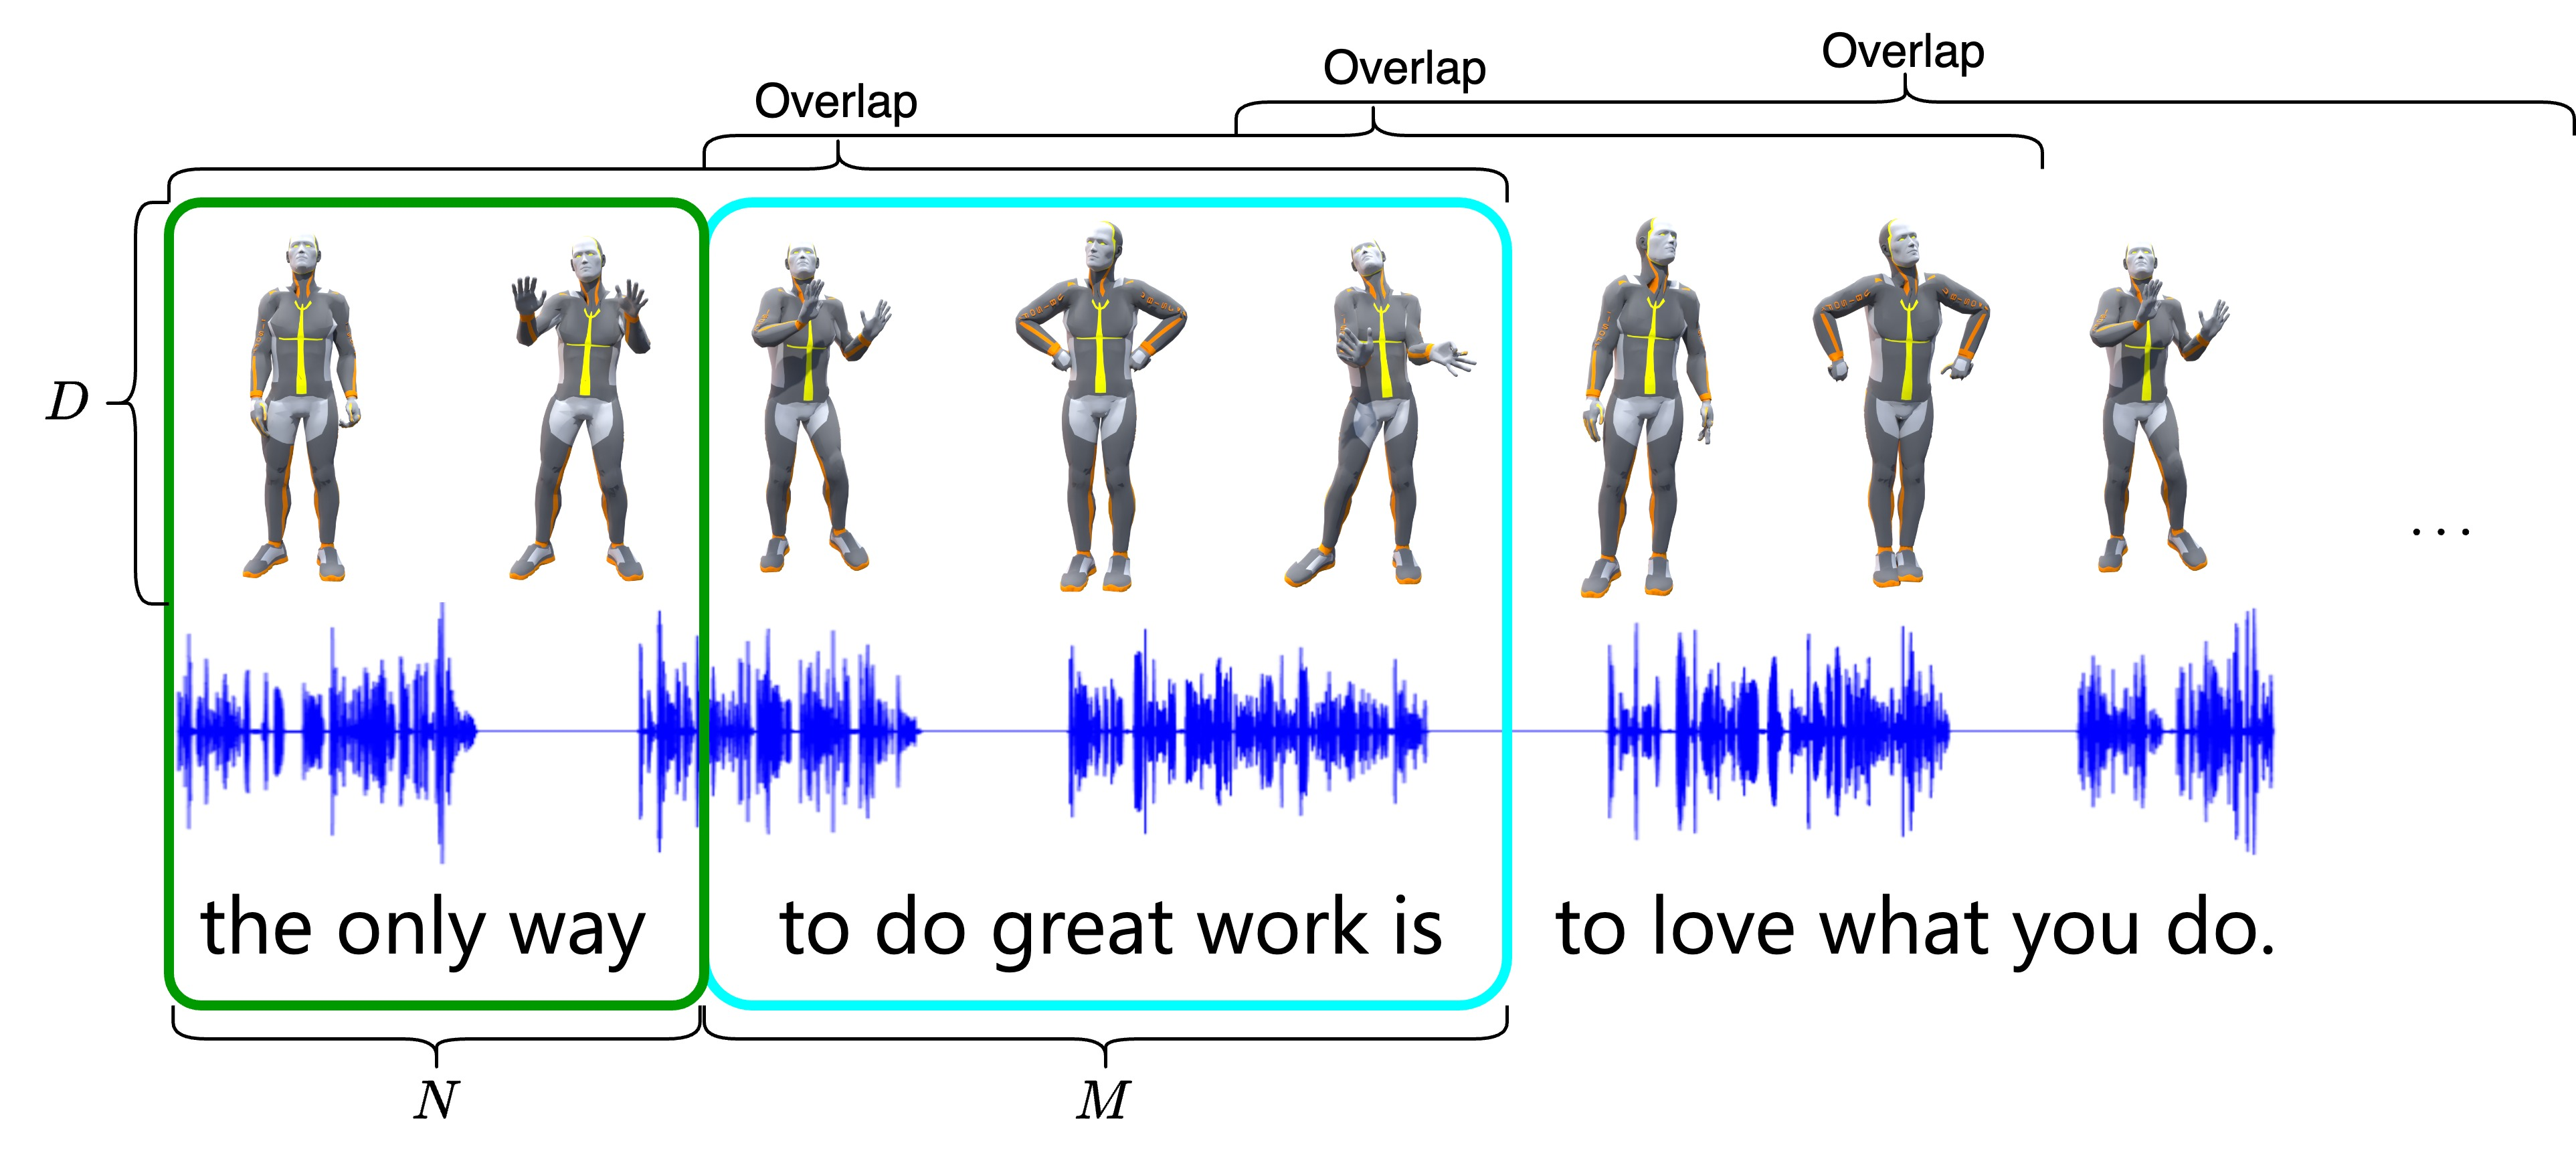
\includegraphics[width=\linewidth]{GestureSeries.jpg}
	\caption{Minh hoạ một chuỗi cử chỉ, ta lấy $N$ frame đầu làm cử chỉ khởi tạo $\mathbf{s}$ (seed gesture) và $M$ khung hình còn lại làm cử chỉ để học}
	\label{fig:GestureSeries}
\end{figure}


Quá trình xử lý dữ liệu được trình bày đầy đủ ở phụ lục \ref{Appendix2}.


%Quá trình chuyển từ không gian Eule sang không gian Quaternion được minh hoạ ở phụ lục \ref{}
%Chuỗi waveform sẽ được cắt thành các đoạn chồng nhau, áp dụng Hamming windows, và áp dụng thuật toán fast fourier transform để biến đổi chuỗi âm thanh thành các hệ số thể hiện cường độ của các tần số trong chuỗi âm thanh, các hệ số này được làm tròn thành các đoạn tần số (frequency bins), các đoạn hệ số này được chuẩn hoá theo hệ cơ số log để tương ứng với cảm nhận của tai người để có được đặc trưng MFCC $\mathbf{a} \in \mathbb{R}^{\text{size} \times \mathcal{C}}$ trong đó $\mathcal{C}=13$ là số frequency bins. 


% \begin{figure}
%     \centering
%     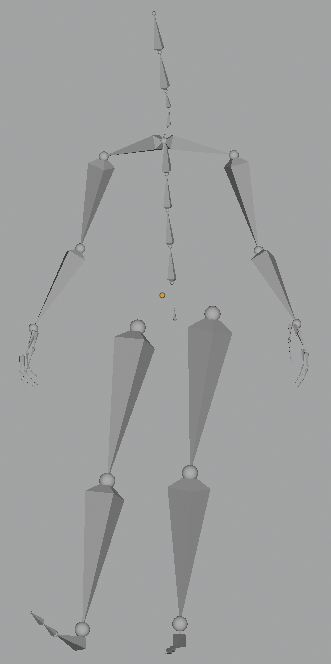
\includegraphics[width=3cm]{images/gesture_sample.png}
%     \caption{Minh họa cử chỉ}
%     \label{fig:gesture_sample}
% \end{figure}

\section{Các khó khăn cần giải quyết}

Có rất nhiều khó khăn trong việc xây dựng một mô hình có thể học được các đăng trưng cử chỉ hội thoại như con người 
%theo thời gian thực:

Thứ nhất, \textit{dữ liệu không đủ nhiều và chất lượng}, chi phí để tạo ra một bộ dữ liệu trong ngành công nghiệp Motion Capture có chất lượng và quy mô lớn để ứng dụng vào trong thực tế là rất lớn.

Thứ hai, \textit{sự thiếu đồng nhất của về ngữ cảnh của các loại dữ liệu}, các bộ dữ liệu về văn bản thường rất nhiều hơn so với giọng nói và cũng không thể biết được văn bản đó được tạo bởi người nào, sự đồng bộ giữa giọng nói và cảm xúc lúc nói cũng thiếu trong việc tạo tập dữ liệu. Ngoài ra, các dữ liệu văn bản lại được nói bởi rất nhiều người khác nhau và ở nhiều nội dung và chủ đề khác nhau.
 
Thứ ba, \textit{sự phân bố không cân xứng về  dữ liệu giữa các loại đăng trưng cần học}. Các dữ liệu dùng cho nghiên cứu cử chỉ hiện nay thường tập trung vào ngôn ngữ Tiếng Anh, các cử chỉ có sự phân bố không cân xứng giữa khi nói, khi hỏi, khi im lặng.

Thứ tư, \textit{chi phí tính toán với nhiều loại dữ liệu của mô hình rất lớn}. Với đầu vào của mô hình gồm rất nhiều loại dữ liệu khác nhau như văn bản, tiếng nói và điểm 3D, nên cần rất nhiều lớp encode cho từng loại dữ liệu cũng là rào cản không nhỏ bởi chi phí tính toán khi huấn luyện và khi suy luận. Nếu giảm thông tin dữ liệu đầu vào cũng sẽ giảm kết quả suy luận của mô hình khi sinh cử chỉ.

Cuối cùng, \textit{các bước xử lý phải yêu cầu tuần tự}, cách hiệu quả nhất để con người tương tác với máy tính là thông qua giọng nói và nhập từ bàn phím, tuy nhiên việc xử lý được văn bản và giọng nói để làm đầu vào cho mô hình phải thực hiện tuần tự, độ trễ để có thể suy luận trong sản phẩm thực tế cũng là một vấn đề bởi người dùng không thể đợi lâu để nhận được kết quả cử chỉ và từ cử chỉ đó biểu diễn lên máy tính bằng kỹ thuật đồ họa máy tính.


\section{Đóng góp dự kiến}

\begin{itemize}
	\item Dựa trên tập dữ liệu có sẵn, chúng tôi chuyển âm thanh của dữ liệu thành văn bản, và dùng văn bản đó để làm dữ liệu huấn luyện mới.
%	\item Tích hợp đặc trưng văn bản vào mô hình DiffuseStyleGesture:** Chúng tôi cải tiến DiffuseStyleGesture bằng cách đưa thông tin văn bản vào quá trình khử nhiễu có điều kiện, giúp hệ thống sinh ra các cử chỉ chi tiết và phù hợp hơn với nội dung hội thoại.
	
	
	\item Dựa trên mô hình cơ bản DiffuseStyleGesture, chúng tôi mở rộng thêm đặc trưng văn bản trong quá trình khử nhiễu có điều kiện.
	
	\item Chúng tôi sử dụng Unity để render, trích xuất dữ liệu và trực quan hoá kết quả sinh cử chỉ.
	
	\item Chúng tôi xây dựng hệ thống kết xuất, và minh hoạ chương trình bằng Unity
	
	
	
%	với thông tin thời gian cho việc sinh cử chỉ kèm theo lời nói dựa trên âm thanh. Nhờ mô hình diffusion, chúng tôi có thể kiểm soát một cách linh hoạt cử chỉ được sinh ra, ví dụ: chỉnh sửa phong cách của cử chỉ, thiết lập cử chỉ khởi tạo, và sinh cử chỉ đa dạng.
	
%	\item Chúng tôi sử dụng cross-local attention và self-attention để để học được bối cảnh và những quan hệ giữa cử chỉ và lời nói.
%	
%	\item Các thử nghiệm mở rộng chỉ ra rằng mô hình của chúng tôi có thể sinh ra cử chỉ giống người, phù hợp với lời nói (speech-appropriateness), phù hợp với cảm xúc (style-appropriateness) vượt trội so với các phương pháp sinh cử chỉ hiện có.
\end{itemize}



%\item **Sử dụng Unity để render, trích xuất dữ liệu và trực quan hoá kết quả sinh cử chỉ:** Chúng tôi triển khai Unity như một công cụ trực quan hóa để mô phỏng và hiển thị kết quả của hệ thống sinh cử chỉ. Với các tính năng mô phỏng 3D mạnh mẽ, Unity cho phép chúng tôi kiểm nghiệm và đánh giá hiệu quả của các cử chỉ được sinh ra từ mô hình, đồng thời hỗ trợ trực quan hóa các đặc trưng chuyển động của cử chỉ. Hệ thống cũng sẽ được phát triển để cho phép dễ dàng trích xuất dữ liệu cử chỉ và so sánh kết quả trực quan giữa các mô hình khác nhau, giúp nâng cao tính khả thi và giá trị thực nghiệm của hệ thống.
%
%\item **Xây dựng hệ thống kết xuất và minh hoạ chương trình bằng Unity:** Ngoài việc render và trực quan hóa kết quả sinh cử chỉ, chúng tôi phát triển hệ thống kết xuất hoàn chỉnh, bao gồm các thành phần giúp dễ dàng minh hoạ quá trình sinh cử chỉ theo từng giai đoạn. Hệ thống này không chỉ cung cấp công cụ để kiểm nghiệm chất lượng cử chỉ sinh mà còn giúp mô tả rõ ràng từng bước trong quá trình sinh cử chỉ, từ giai đoạn tiền xử lý dữ liệu, khử nhiễu, đến việc ứng dụng các đặc trưng văn bản và âm thanh để tạo ra cử chỉ. Điều này sẽ làm tăng tính minh bạch và khả năng giải thích của hệ thống, đồng thời hỗ trợ các nhà nghiên cứu và người dùng dễ dàng quan sát và hiểu sâu hơn về các bước sinh cử chỉ. 

%\begin{itemize}
%\item Chúng tôi mở rộng mô hình diffusion với thông tin thời gian cho việc sinh cử chỉ kèm theo lời nói dựa trên âm thanh. Nhờ mô hình diffusion, chúng tôi có thể kiểm soát một cách linh hoạt cử chỉ được sinh ra, ví dụ: chỉnh sửa phong cách của cử chỉ, thiết lập cử chỉ khởi tạo, và sinh cử chỉ đa dạng.
%
%\item Chúng tôi sử dụng cross-local attention và self-attention để để học được bối cảnh và những quan hệ giữa cử chỉ và lời nói.
%
%\item Các thử nghiệm mở rộng chỉ ra rằng mô hình của chúng tôi có thể sinh ra cử chỉ giống người, phù hợp với lời nói (speech-appropriateness), phù hợp với cảm xúc (style-appropriateness) vượt trội so với các phương pháp sinh cử chỉ hiện có.
%\end{itemize}


% Đầu vào của hệ thống trí tuệ nhân tạo cho việc sinh cử chỉ bao gồm: 

% Tức đã có input (audio/text) sang output (text). Nhưng chưa có từ text sang 1 visual.

% Để xây dựng 1 virtual human assitant mà tương tác được cần sinh ra Output:

% - Hình ảnh: text to visual: 3D scan da người, các texture, mesh và quan trọng nhất là cử chỉ của người đó.

% - Âm thanh: text to speech.

% Để học được các cử chỉ thì dữ liệu đầu vào dĩ nhiên bao gồm các keypoint 3D về cử chỉ, dữ liệu cử chỉ bao gồm cử chỉ của cơ thể ($\Omega_{\text{Body}}$) cử chỉ của bàn tay ($\Omega_{\text{Hand}}$) và biểu cảm khuôn mặt ($\Omega_{\text{Facial}}$).

% $$
% \Omega = \{ \Omega_{\text{Speaker_ID}}; \Omega_{\text{Emotion_ID}}; \Omega_{\text{Text}}; \Omega_{\text{Speech}}; \\
% \Omega_{\text{Facial}}; \Omega_{\text{Hand}}; \Omega_{\text{Body}}
% \} 
% $$

% \section{Bài toán sinh cử chỉ}

%Đầu vào của mô hình sinh cử chỉ là chuỗi văn bản (text), chuỗi lời nói (speech) và tọa độ cử chỉ khởi tạo, với đầu ra là chuỗi cử chỉ được sinh ra tương ứng với văn bản và lời nói tương ứng.

%là các keypoint chuyển động trên không gian tọa độ 3 chiều của cử chỉ cơ thể (\textbf{body gesture}), cử chỉ bàn tay (\textbf{hand gesture}) và biểu cảm khuôn mặt (\textbf{facial expression}), tương ứng từng cử chỉ là văn bản (\textbf{text}) và giọng nói (\textbf{speech}). Mỗi người đều có phong cách cử chỉ khác nhau và cảm xúc lúc nói khác nhau nên cũng cần phải có thêm thông tin về người nói (\textbf{speaker identity}) và cảm xúc lúc nói (\textbf{emotions}) tương ứng. 
%
%Kết quả đầu ra của việc sinh cử chỉ là chuỗi các cử chỉ (gesture), với mỗi cử chỉ là tập các điểm trong tọa độ 3D ( bao gồm vị trí ($x, y, z$) và góc quay ($r_{x}, r_{y}, r_{z}$ ) ) như hình minh họa 




% Ngôn ngữ để viết và trình bày báo cáo khóa luận tốt nghiệp, đồ án tốt nghiệp, thực tập tốt nghiệp (sau đây gọi chung là báo cáo) là tiếng Việt hoặc tiếng Anh. 
% Trường hợp chọn ngôn ngữ tiếng Anh để viết và trình bày báo cáo,  sinh viên cần có đơn đề nghị, được cán bộ hướng dẫn (CBHD) đồng ý và nộp cho bộ phận Giáo vụ của Khoa vào thời điểm đăng ký đề tài để xin ý kiến.
% Báo cáo viết và trình bày bằng tiếng Anh phải có bản tóm tắt viết bằng tiếng Việt.


%Tóm tắt luận văn được trình bày nhiều nhất trong 24 trang in trên hai mặt giấy, cỡ chữ Times New Roman 11 của hệ soạn thảo Winword hoặc phần mềm soạn thảo Latex đối với các chuyên ngành thuộc ngành Toán.

%Mật độ chữ bình thường, không được nén hoặc kéo dãn khoảng cách giữa các chữ.
%Chế độ dãn dòng là Exactly 17pt.
%Lề trên, lề dưới, lề trái, lề phải đều là 1.5 cm.
%Các bảng biểu trình bày theo chiều ngang khổ giấy thì đầu bảng là lề trái của trang.
%Tóm tắt luận án phải phản ảnh trung thực kết cấu, bố cục và nội dung của luận án, phải ghi đầy đủ toàn văn kết luận của luận án.
%Mẫu trình bày trang bìa của tóm tắt luận văn (phụ lục 1).
